\documentclass[10pt,a4paper]{scrartcl}
\usepackage[utf8]{inputenc}
\usepackage{amsmath}
\usepackage{amsfonts}
\usepackage{pgfpages}
\usepackage{amssymb}
\usepackage[utf8]{inputenc}
\usepackage[ngerman]{babel}
\usepackage[autostyle]{csquotes}
\usepackage[left=2.54cm,right=2.54cm,top=2.54cm,bottom=2.54cm]{geometry}

\author{Leonard Hackel, Jochen Jacobs, Niklas Schelten}
\title{Manual zur Benutzung des 3D-Druckers}
\begin{document}
\maketitle
\begin{center}
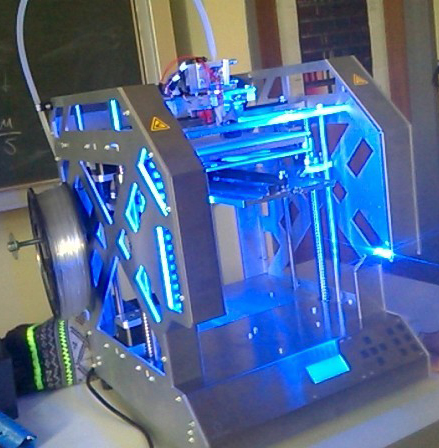
\includegraphics[scale=0.75]{res/31_1.jpg}
\end{center}
\pagebreak
\tableofcontents
\pagebreak
%---------------------------Jochen----------------------------------------------
\section{Erstellen von 3D Objekten}
\pagebreak
%---------------------------Jochen----------------------------------------------
\section{Der Druck}
% neuen Drucker hinzufügen/vor der ersten Nutzung
Da Cura den RF1000 nicht als Standard dabei hat, muss dieser vorher als neuer Drucker hinzugefügt werden. Dazu muss man unter \textit{Machine}, \textit{Add new machine...} dieser neu erstellt werden. Da er keine Voreinstellung ist, muss im \textit{Configuration Wizard} \textit{Other} gewählt werden, ebenso wie unter \textit{Other machine information} \textit{Custom...} ausgewählt sein muss. Nun kann man Namen (\textit{Machine name}), also RF1000, und Größe unter \textit{width}, \textit{depth} und \textit{height} einstellen (für den RF1000 245,235,200 mm in dieser Reihenfolge). \textit{Nozzle Size} ist standardmäßig 0.5 und für den RF1000 korrekt. Zusätzlich muss die Option \textit{Heated Bed} ausgewählt werden, die Option \textit{Bed center [...]} ist nicht zutreffend.\\
Danach müssen die anderen Einstellungen, welche sich auf der SD-Karte finden lassen, geladen werden. Dazu muss unter \textit{File}, \textit{Open Profile...} die Datei \textit{Settings.ini} geladen werden. Danach ist der RF1000 als Drucker eingestellt und kann für den Druck konfiguriert werden.\\
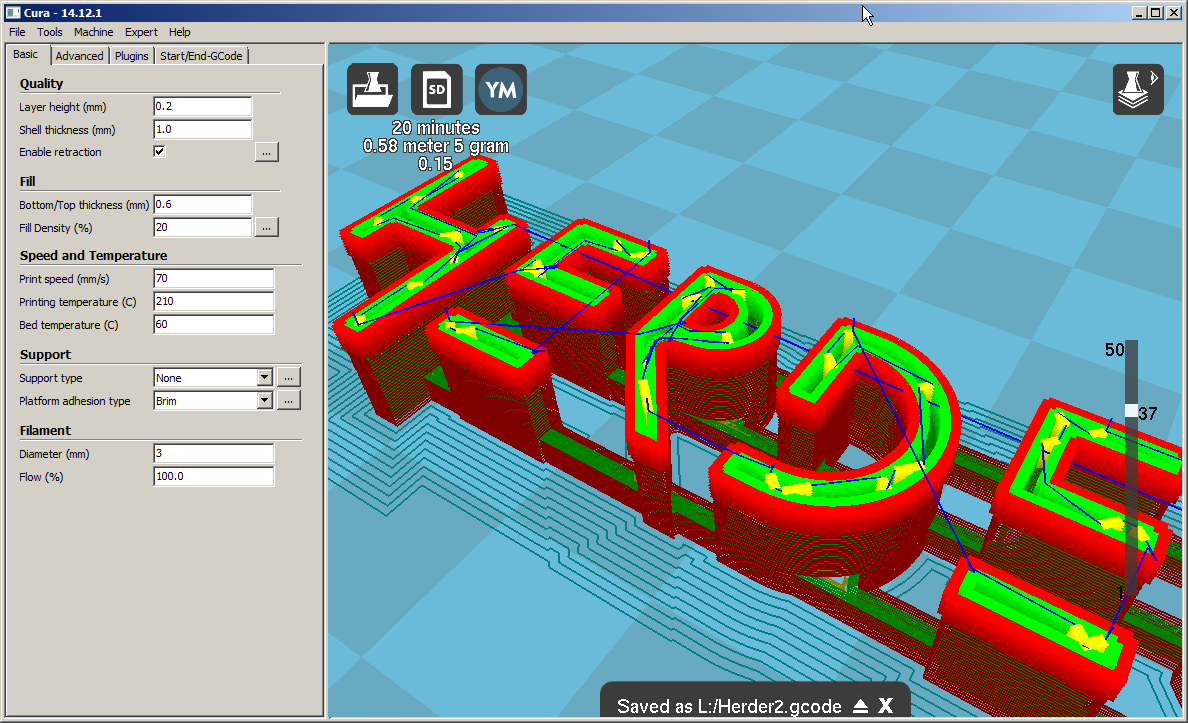
\includegraphics[scale=0.4]{res/Cura-window.png}\\

Um nun in diese Ansicht zu gelangen, muss man bei Cura im Reiter \textit{Expert} unter \textit{Switch to full settings} die Ansicht ändern. Dabei verschwinden die Schnelleinstellungen und diese Ansicht erscheint. Das hat den Vorteil, dass die Einstellungen viel genauer vorgenommen werden können.\\
Das Vorschaufenster bei Cura besteht aus zwei großen Teilen. Auf der linken Seite sind die Einstellungen, auf der rechten ist eine 3D-Ansicht des Objektes. Dabei sind verschiedene Strecken in verschiedenen Farben angezeigt. Innenstrecken sind dabei grün, Druckstrecken, die später Außenflächen ergeben, sind rot, und Strecken, welche der Druckkopf zurücklegt, dabei aber nicht druckt, sind dünner und blau. In gelb dargestellt sind diejenigen Strecken, die später Füllung sind.\\
Die meisten Einstellungen sind selbsterklärend. So gibt die \textit{Layer heigt} an, wie hoch die einzelnen Drucklagen sind, wodurch damit auch die Anzahl der Lagen bestimmt wird. \textit{Shell thickness} gibt an, wie viele Spuren außen gedruckt werden, bevor der Bereich als Innenraum gilt und nur zu einem bestimmten Prozentsatz gefüllt wird. dieser ist unter \textit{Fill Density} einstellbar. So wie \textit{Shell thickness} die Dicke der seitlichen Außenhaut angibt, gibt \textit{Bottom/Top thickness} dies für die oberen und unteren Schichten an.\\
\textit{Print speed} gibt an, wie schnell sich der Druckkopf relativ zu der Heizplatte bewegt, wenn er druckt (unter \textit{Advaced} gibt es noch andere Bewegungsarten). Hierbei gilt generell, dass eine geringere Geschwindigkeit die Qualität, allerdings auch die Druckzeit erhöht, wodurch ein geeignetes Mittelmaß zu finden ist. \textit{Printing temperature} und \textit{Bed temperature} sind von dem Druckmaterial abhängig, für PLA empfiehlt sich 210/60. Generell empfehlen wir die oben gezeigten Werte für die bisher genannten Einstellungen bei einem Druck mit PLA.\\
Unter \textit{Support} finden sich Einstellungen, die den Drucker bei schwereren Aufgaben wie Überhängen unterstützen. Sollte das Objekt Überhänge haben, empfehlen wir den \textit{Support type} \textit{Touching buildplate}, wenn es sich aber nur um kleine oder steile Überhänge handelt, ist ein Support nicht empfehlenswert (ab 60\% ist Support benötigt, ansonsten muss von Fall zu Fall unterschieden werden). Als \textit{Platform adhesion type} empfehlen wir einen \textit{Brim} der Breite 10, damit sich der Drucker \enquote{eindrucken} kann, wodurch Filamentaussetzer und Stotterer vermieden werden. Bei Objekten, welche leicht umfallen oder wackeln, ist ein \textit{Raft} zu empfehlen, da es den Druck stabilisiert. Allerdings kostet der Druck eines solchen viel Zeit.\\
\textit{Filament}-Settings sollten bei 3 (\textit{Diameter}) und 100(\textit{Flow}) gelassen werden.
\pagebreak
%---------------------------Niklas----------------------------------------------
\section{Probleme beim Drucken}
\iffalse
Probleme:
-Aus Extruder kommt nichts raus
-Druck hält nicht
-Extruder kratzt auf Heatbed
-Filament bricht
-Extruder verstopft (sollte bei Beachtung der anderen Fehler nicht passiere)
\fi

Beim Drucken von 3D Objekten können viele verschieden und unterschiedlich schwerwiegende Probleme auftreten. Hier sind die jeningen gelistet, dioe uns am häufigsten passiert sind:\\
\begin{description}
\item \textbf{Aus dem Extruder kommt nichts heraus.}\\
Für dieses Problem kann es verschiedene Ursachen geben:
\begin{itemize}
\item \textit{Es ist kein Filament eingelegt}\\
In diesem Fall ist der Extruder auf die für das gewünschte Filament benötigte Temperatur (PLA $210^\circ$C) zu erhitzen. Wenn dieser heiß ist kann man das Filament in den Extruder einführen und den Extrudervorschub manuell erhöhen bis unten Filament heraus tropft. Dies kann lange dauern, wenn der Extruder vorher leer war.\\
\textbf{ACHTUNG: Bei zu schnellem Vorschieben kann es passieren, dass das Filament sich nicht schnell genug erhitzt und dann den Extruder verstopft.}

\item \textit{Es ist vorher Filament aus dem Extruder gelaufen, ohne, dass welches nachgechoben wurde}\\

\end{itemize}
\end{description}
\end{document}